\begin{figure}[H]
\centering
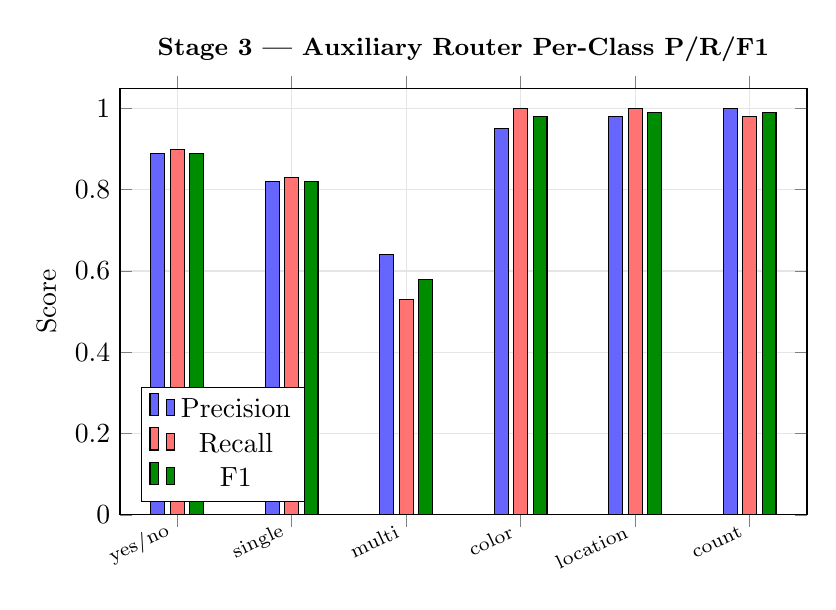
\begin{tikzpicture}
\begin{axis}[ybar, width=0.85\linewidth, height=7cm,
    title={\textbf{Stage 3 --- Auxiliary Router Per-Class P/R/F1}},
    title style={font=\small\bfseries}, ylabel={Score}, ymin=0, ymax=1.05,
    symbolic x coords={yes/no,single,multi,color,location,count}, xtick=data,
    x tick label style={rotate=25, anchor=east, font=\scriptsize},
    legend pos=south west, bar width=5pt, grid=major, grid style={gray!20}]
\addplot[fill=blue!60] coordinates {(yes/no,0.890) (single,0.820) (multi,0.640) (color,0.950) (location,0.980) (count,1.000)};
\addlegendentry{Precision}
\addplot[fill=red!55] coordinates {(yes/no,0.900) (single,0.830) (multi,0.530) (color,1.000) (location,1.000) (count,0.980)};
\addlegendentry{Recall}
\addplot[fill=green!55!black] coordinates {(yes/no,0.890) (single,0.820) (multi,0.580) (color,0.980) (location,0.990) (count,0.990)};
\addlegendentry{F1}
\end{axis}\end{tikzpicture}
\caption[Stage 3 per-class router]{Per-class precision, recall, and F1 of the
Stage~3 auxiliary routing head on the test set. Support: yes/no~4657, single~2618, multi~377, color~1429, location~2278, count~4596.}
\label{fig:stage3_per_class}
\end{figure}
